\documentclass{beamer}
\usepackage[british]{babel}        % for german language
\usepackage[utf8]{inputenc}        % for umlauts and other non 7bit ascii things
\usepackage[T1]{fontenc}           % this is needed for correct output of umlauts in pdf
\usepackage{lmodern}               % use a vector based font, not a bitmap based font for T1
\usepackage[stretch=10]{microtype} % improves font placements
\usepackage[autostyle=true,german=quotes]{csquotes}

%\usepackage[backend=biber,style=numeric]{biblatex}
%\addbibresource{master.bib}

\usepackage{mathtools}
\usepackage{amsfonts,amsmath,amssymb,amsthm}
\newcommand\numberthis{\addtocounter{equation}{1}\tag{\theequation}}
\usepackage{ marvosym }
%\usepackage{array, tabularx}
\usepackage{colortbl}
\definecolor{codegray}{rgb}{0.5,0.5,0.5}
\definecolor{backcolour}{rgb}{0.8,0.8,0.8}
\usepackage{graphicx}
\usepackage{subfigure}
\hypersetup{pdfstartview={Fit}}


\newcommand{\E}{\mathbb{E}}
\newcommand{\abs}[1]{\vert{#1}\vert}
\renewcommand{\vec}[1]{\ensuremath{{\bf #1}}}
\newcommand{\dotp}[2]{\ensuremath{\left\langle #1, #2 \right\rangle}}
\newcommand{\st}{\ensuremath{s}}
\newcommand{\mst}{\ensuremath{w}}
\newcommand{\opt}{\text{\textsc{Opt}} }
\newcommand{\myprop}{\ensuremath{\texttt{RVU}}}

\setbeamercolor{postit}{fg=black,bg=yellow}

\title{Fast Convergence of Regularized Learning in Games}
\author{Malte Schledjewski}
\institute{Saarbrücken Graduate School of Computer Science}
\date{2016}

\usetheme{Frankfurt} %Darmstadt

\begin{document}
	
\frame{\titlepage}

\section{Games}

\begin{frame}
	\frametitle{The paper}
	\begin{block}{Fast Convergence of Regularized Learning in Games}
		\begin{itemize}
			\item Vasilis Syrgkanis, Microsoft Research
			\item Alekh Agarwal, Microsoft Research
			\item Haipeng Luo, Princeton University
			\item Robert E. Schapire, Microsoft Research
		\end{itemize}
		published 2015
	\end{block}
\end{frame}


\begin{frame}[c]
	\begin{center}
		\Huge Joshua: Shall we play a game?
	\end{center}
\end{frame}

\subsection{The game}
\begin{frame}
	\frametitle{A little game}
	\begin{itemize}
		\item 4 bidders
		\item 4 items each worth 20
		\item each bidder has no extra value from more than one item
		\item bids are integers in [1,20]
		\item highest bid wins and must be paid
		\item ties are broken arbitrarily 
	\end{itemize}
\end{frame}



\subsection{Intuition}
\begin{frame}
	\frametitle{Basic intuition}
    If players are
		\begin{itemize}
			\item smart,
			\item selfish and
			\item acting independently
		\end{itemize}
		
	we expect\pause
	\begin{figure}[!tbp]
		\centering
		\begin{minipage}[b]{0.4\textwidth}
			\includegraphics[height=3cm]{scrum} \pause
		\end{minipage}
		\hfill
		\begin{minipage}[b]{0.4\textwidth}
			\includegraphics[height=3cm]{Muixeranga2} \pause
		\end{minipage}
	\end{figure}
	
	\begin{itemize}
		\item the dynamics to stabilize and
		\item the utilities to approach a maximum (individually and as a group).
	\end{itemize}
\end{frame}

\subsection{Finite set of strategies}
\begin{frame}
	\frametitle{Finite amount of strategies}
	For a game G of $n$ players:\\
	Each player $i$ has a finite strategy space $S_i$.
	
\pause
	\begin{beamercolorbox}[sep=1em]{postit}
		All combination to bid up to 20 for the four items.
	\end{beamercolorbox}
	\pause
	Utility function $u_i : S_1 \times \ldots \times S_n \rightarrow [0,1]$
	\pause
	\begin{beamercolorbox}[sep=1em]{postit}
		(value - cost) / 20
	\end{beamercolorbox}
\end{frame}



\begin{frame}
	\frametitle{You just made a friend\ldots}
	\begin{columns}[T]
		\begin{column}{.5\textwidth}
			\includegraphics[height=7cm]{adversary} \pause
		\end{column}
		\begin{column}{.5\textwidth}
			\begin{beamercolorbox}[sep=1em]{postit}
				He is mean and simply gives the items to the other three guys.
			\end{beamercolorbox}\pause
			The adversary can choose the worst outcome for you.
			
			\vspace{1em}
			\pause
			So just be a little bit random and don't let the adversary know the result of the random draw.
		\end{column}
	\end{columns}
	
\end{frame}

\subsection{One round}

\begin{frame}
	\frametitle{Repeat and repeat and repeat and\ldots}
	\begin{block}{Mixed strategies}
	\begin{itemize}
		
		\item $ w = (w_1 , \ldots, w_n)$, a profile of mixed strategies with
		\begin{itemize}
			\item $w_i \in \Delta(S_i)$
			\item $w_{i,x}$ is the probability of strategy $x \in S_i$
		\end{itemize}
		%\item  $U_i(w) = \mathbb{E}_{s\sim{}w}[u_i(s)]$, the expected utility of player $i$
		
	\end{itemize}
	\end{block}
	\pause
	\begin{block}{Repetition is good for learning}
		The game G is repeatedly played for T time steps.\\
		For each time step:
		\begin{itemize}
			\item Each player $i$ picks a mixed strategy $\mathbf{w}^t_i \in \Delta(S_i)$ 
			\item Each player observes the expected utility for each strategy $x$: $\mathbf{u}^t_i = (u^t_{i,x})_{x \in S_i} $ with $ u^t_{i,x} = \mathbb{E}_{s_{-i} \sim w^t_{-i}} \left[u_i(x,s_{-i})\right] $
		\end{itemize}
		
		The expected utility for a player $i$ in iteration $t$ is therefore 
		$ \left\langle w^t_{i},u^t_{i}\right\rangle $.
	\end{block}
\end{frame}


\subsection{Regret}

\begin{frame}
	\frametitle{Regret or no regret -- that is the question}
		\begin{block}{Regret}
			\begin{equation*}
			r_i(T) = \sup\limits_{\mathbf{w}^*_i \in \Delta (S_i)} \sum_{t=1}^{T} \left< \mathbf{w}^*_i - \mathbf{w}^t_i, \mathbf{u}^t_i \right>
			\end{equation*}\pause
			\begin{beamercolorbox}[sep=1em]{postit}
				How much could you have gained if you had played the best (up to now) possible mixed strategy? 
			\end{beamercolorbox}
		\end{block}
		\pause
				\begin{block}{No-regret}
					\begin{equation*}
					r_i(T) \in o(T)
					\end{equation*}\pause
					\begin{beamercolorbox}[sep=1em]{postit}
						So your average regret converges to 0.
					\end{beamercolorbox}
				\end{block}
\end{frame}


\subsection{No regret}
\begin{frame}
	\frametitle{No-regret suits you}
	Assume all players chose $\mathbf{w}^t_i$ based on a no-regret learning algorithm.
	
	Suitable because:
	\begin{itemize}
		\item regret-bounds hold against adversarial environments
		\item each player's utility approaches optimality
		\item when played against each other
		\begin{itemize}
			\item the social welfare reaches an approximate optimum
			\item the mixed strategies converge to an equilibrium based with rates based on the regret bounds
		\end{itemize} 
		\item there are well-known families of no-regret algorithms, for which the average regret vanishes at the worst-case rate of $O(1/\sqrt{T})$, which is unimprovable against fully adversarial environments.
	\end{itemize}
\end{frame}


\subsection{No regret}
\begin{frame}
	\frametitle{Follow the white rabbit -- oh, I meant the leader}
	\begin{block}{Follow the Leader}
		Because you regret one mixed strategy the most, just play it in the next round.
	\end{block}
	\pause
	\begin{beamercolorbox}[sep=1em]{postit}
		What could go wrong?
	\end{beamercolorbox}
	\pause
	\begin{block}{Bad example}
		\begin{align*}
			 f(T) =
			\begin{cases}
			-0.5       & \quad \text{if } t = 1 \\
			1  & \quad \text{if } t \text{ is even}\\
			-1  & \quad \text{if } t > 1 \text{ and } t \text{ is odd}\\
			\end{cases}
		\end{align*}
		\begin{beamercolorbox}[sep=1em]{postit}
			FTL predicts exactly the opposite.\\
			Regret compared to constant 0 prediction grows linear.
		\end{beamercolorbox}
	\end{block}
\end{frame}

%stability
%regret upper bounded by w-w






\subsection{Smoothness}
\begin{frame}
	\frametitle{Smooth games}
	\begin{block}{Smooth game}
		A game is
		$(\lambda,\mu)$-smooth if there exists a strategy profile
		$\vec{\st}^*$ such that for any strategy profile $\vec{\st}$:
		
		\begin{equation*}
		\sum_{i\in N} u_i(\st_i^*,\vec{\st}_{-i}) \geq \lambda \opt - \mu
		W(\vec{\st})
		\end{equation*}
	\end{block}
	\pause
	\begin{block}{}
		In a $(\lambda,\mu)$-smooth game, if each player $i$ suffers regret at
		most $r_i(T)$, then:
		\begin{equation*}
		\frac{1}{T} \sum_{t=1}^{T}
		W(\vec{\mst}^t) \geq \frac{\lambda}{1+\mu} \opt
		- \frac{1}{1+\mu}\frac{1}{T}\sum_{i\in N} r_i(T)
		\end{equation*}
	\end{block}
\end{frame}


\section{Contributions}
% we only focus on Social Welfare
% previous O
\subsection{Contributions}
\begin{frame}
	\frametitle{Contributions}
	For a certain class of no-regret dynamics in smooth games, when played against each other:
	\begin{itemize}
		\item\alert<3>{ The average welfare converges to approximate optimum at the rate $O(1/T)$ instead of $O(1/\sqrt{T})$.}
		\item The average welfare is at least $ (\lambda / (1 + \mu)) \text{OPT} - O(1/T) $.
		\item Each player's average regret converges to zero at rate $O(T^{-3/4})$.
	\end{itemize}\pause
	A black-box reduction that preserves the rate in favourable environments and maintains $\tilde{O}(1/\sqrt{T})$ against adversarial environments.
\end{frame}




\section[A class of no-regret dynamics]{A special class of no-regret dynamics}
\subsection{RVU property}
% what do the terms mean

\begin{frame}
	\frametitle{RVU property}
	\begin{block}{RVU -- Regret bounded by Variation in Utilities}
		A vanishing regret algorithm has the RVU property with parameters $\alpha>0$ and $0<\beta\leq\gamma$ and a pair of dual norms $(\|\cdot\|, \|\cdot\|_*)$ if for any sequence of utilities $\vec{u}^1, \vec{u}^2, \ldots, \vec{u}^T$ the regret is bounded as 
		\begin{equation*}
		\sum_{t=1}^{T} \dotp{\vec{w}^*- \vec{w}^t}{\vec{u}^t} \leq \alpha
		+\beta \sum_{t=1}^{T} \| \vec{u}^t - \vec{u}^{t-1}\|_*^2 -
		\gamma\sum_{t=1}^{T} \|\vec{w}^{t} - \vec{w}^{t-1}\|^2
		\end{equation*}  
	\end{block}
	
	\begin{block}{Dual to a norm}
		The dual to a norm
		$\|\cdot\|$ is defined as $\|u\|_* = \sup_{\|w\| \leq 1}
		\dotp{w}{u}$.
	\end{block}
\end{frame}

\subsection{The middle term}
% explain dual norm -> max

\begin{frame}
	\frametitle{An observation on $ \| \vec{u}^t - \vec{u}^{t-1}\|_*^2 $}
	We will now use the $\ell_1$ norm.
	
	\begin{align*}
		\onslide<1->{&\| \vec{u}^t_i - \vec{u}^{t-1}_i \|_*
	   =\sup_{\|w\| \leq 1} \dotp{w}{\vec{u}^t_i - \vec{u}^{t-1}_i} 
	   =\max_{x \in S_i} \left| u_{i,x}^t - u_{i,x}^{t-1} \right|  \\}
	   \onslide<2->{=&\max_{x \in S_i} \left| \E_{\vec{s}_{-i}\sim \vec{w}_{-i}^t}[u_i(x,\vec{s}_{-i})] - \E_{\vec{s}_{-i}\sim \vec{w}_{-i}^{t-1}} [u_i(x,\vec{s}_{-i})] \right| \\}
	   \onslide<3->{=&\max_{x \in S_i} \left| \sum_{\tilde{s} \in \vec{s}_{-i}} u_i(x,\tilde{s}) ( \text{Prob}^t(\tilde{s}) - \text{Prob}^{t-1}(\tilde{s}))   \right|\\}
	   \onslide<4->{\leq&\max_{x \in S_i} \sum_{\tilde{s} \in \vec{s}_{-i}} u_i(x,\tilde{s})  \left| ( \text{Prob}^t(\tilde{s}) - \text{Prob}^{t-1}(\tilde{s}))   \right|\\}
	   \onslide<5->{\leq& \sum_{\tilde{s} \in \vec{s}_{-i}} \left| \prod_{j\neq i} \mst_{j,\tilde{s}_j}^t - \prod_{j\neq i}\mst_{j,\tilde{s}_j}^{t-1}\right| }
	   \onslide<6->{\leq \sum_{j\neq i} \|
	   \vec{\mst}_j^t-\vec{\mst}_j^{t-1}\|}
	\end{align*}
\end{frame}

\section[Social welfare]{Fast convergence of social welfare}
  \subsection{Theorem 4} %with proof
  \begin{frame}
  	\frametitle{Fast convergence of social welfare}
	
	\begin{block}{Fast convergence of social welfare}
		Suppose that the algorithm of each player $i$ satisfies the \myprop~property
		with parameters $\alpha, \beta$ and $\gamma$ such that
		$\beta\leq \gamma/(n-1)^2$ and $\|\cdot\| = \|\cdot\|_1$. \\
		Then $\sum_{i\in N} r_i(T) \leq \alpha n$ and therefore the social welfare converges at a rate of $O(1/T)$.
	\end{block}
	\pause
	\begin{align*}
	\onslide<2->{&\text{Our previous observation: } \| \vec{u}^t - \vec{u}^{t-1} \|_*
	\leq \sum_{j\neq i} \| \vec{\mst}_j^t-\vec{\mst}_j^{t-1}\|\\
	&\sum_{i\in N} \|\vec{u}_i^t-\vec{u}_i^{t-1}\|_*^2
	\leq \sum_{i\in N} \left(\sum_{j\neq i} \| \vec{\mst}_j^t-\vec{\mst}_j^{t-1}\|\right)^2 \\}
	\onslide<3->{&\leq \sum_{i\in N}  \left((n-1) \sum_{j\neq i} \| \vec{\mst}_j^t-
	\vec{\mst}_j^{t-1}\|^2 \right)
	= (n-1)^2 \sum_{i\in N} \| \vec{\mst}_i^t-
	\vec{\mst}_i^{t-1}\|^2}
	\end{align*}

  \end{frame}
  
    \begin{frame}
    	\frametitle{Proof, continued}
    	

    	\begin{align*}
    	\onslide<1->{\sum_{i\in N} r_i(T) &\leq 
    	\sum_{i\in N} \left( \alpha
    	+\beta \sum_{t=1}^{T} \| \vec{u}^t_i - \vec{u}^{t-1}_i\|_*^2 -
    	\gamma\sum_{t=1}^{T} \|\vec{w}^{t}_i - \vec{w}^{t-1}_i \|^2 \right)\\}
    	\onslide<2->{&=\alpha n + \sum_{t=1}^{T} \left( \beta \sum_{i\in N} \| \vec{u}^t_i - \vec{u}^{t-1}_i\|_*^2
    	- \gamma \sum_{i\in N} \|\vec{w}^{t}_i - \vec{w}^{t-1}_i \|^2  \right)\\}
    	\onslide<3->{\leq \alpha &n + \sum_{t=1}^{T} \left( \beta (n-1)^2 \sum_{i\in N} \| \vec{\mst}_i^t-
    	\vec{\mst}_i^{t-1}\|^2
    	- \gamma  \sum_{i\in N} \|\vec{w}^{t}_i - \vec{w}^{t-1}_i \|^2  \right)\\}
    	\onslide<4->{&\leq \alpha n + \sum_{t=1}^{T} \left( \left(  \beta (n-1)^2 
    	- \gamma \right)  \sum_{i\in N}\|\vec{w}^{t}_i - \vec{w}^{t-1}_i \|^2 \right)\\}
    	\onslide<5->{&\leq \alpha n + \sum_{t=1}^{T} \left( \left(  \frac{\gamma}{(n-1)^2}  (n-1)^2 
    	- \gamma \right)  \sum_{i\in N}\|\vec{w}^{t}_i - \vec{w}^{t-1}_i \|^2 \right)\\
    	&\leq \alpha n}
    	\end{align*}
    	
    \end{frame}
  
\section[OFRL]{Optimistic Follow the Regularized Leader} % a lot

\begin{frame}
	\frametitle{Placeholder}
\end{frame}

%\section{Robustness against adversary}

\section{Experiment}
% fast convergence, stable and better equilibrium (higher welfare)
\subsection{Experimental setting}
\begin{frame}
	\frametitle{The experiment}
	\begin{itemize}
		\item 4 bidders
		\item 4 items each worth 20
		\item each bidder has no extra value from more than one item
		\item bids are integers in [1,20]
		\item highest bid wins and must be paid
	\end{itemize}
\end{frame}

\subsection{Results I}
\begin{frame}
	\frametitle{Results I}
	\begin{figure}[!t]
		\centering
		\subfigure{
			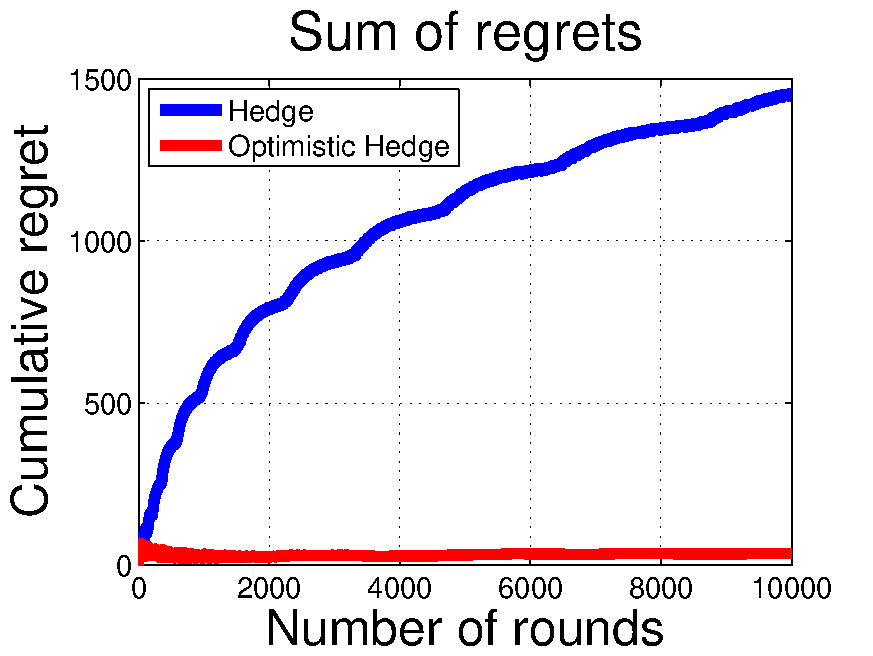
\includegraphics[width=0.4\textwidth,height=0.3\textwidth]{sum_regret.pdf}
		}
		\quad
		\subfigure{
			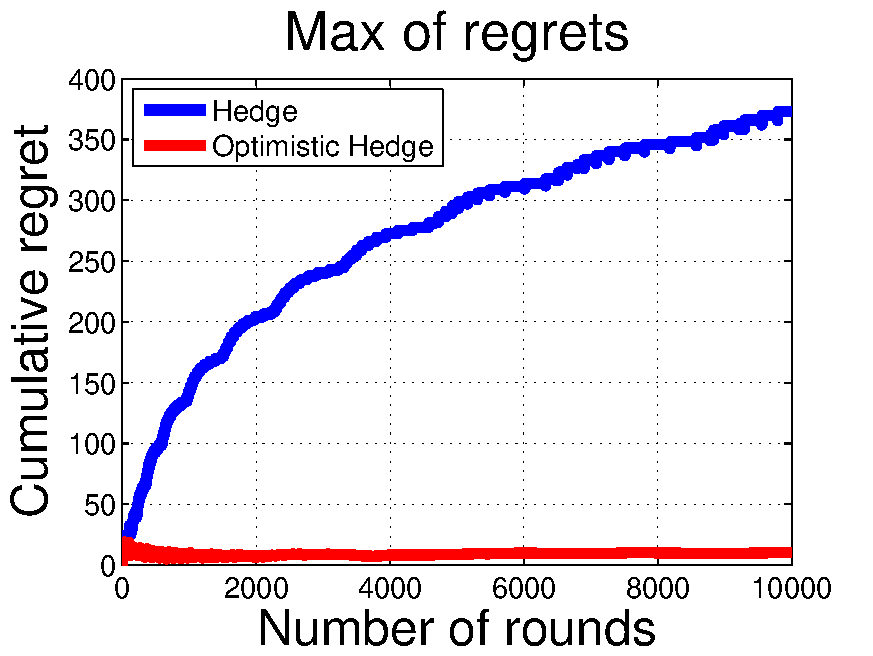
\includegraphics[width=0.4\textwidth,height=0.3\textwidth]{max_regret.pdf}
		}
		\caption{Maximum and sum of individual regrets over time under the
			Hedge (blue) and \mbox{Optimistic Hedge} (red) dynamics.}\label{fig:regrets}
	\end{figure}
\end{frame}

\subsection{Results II}
\begin{frame}
	\frametitle{Results II}
	\begin{figure}[!t]
		\centering
		\subfigure{
			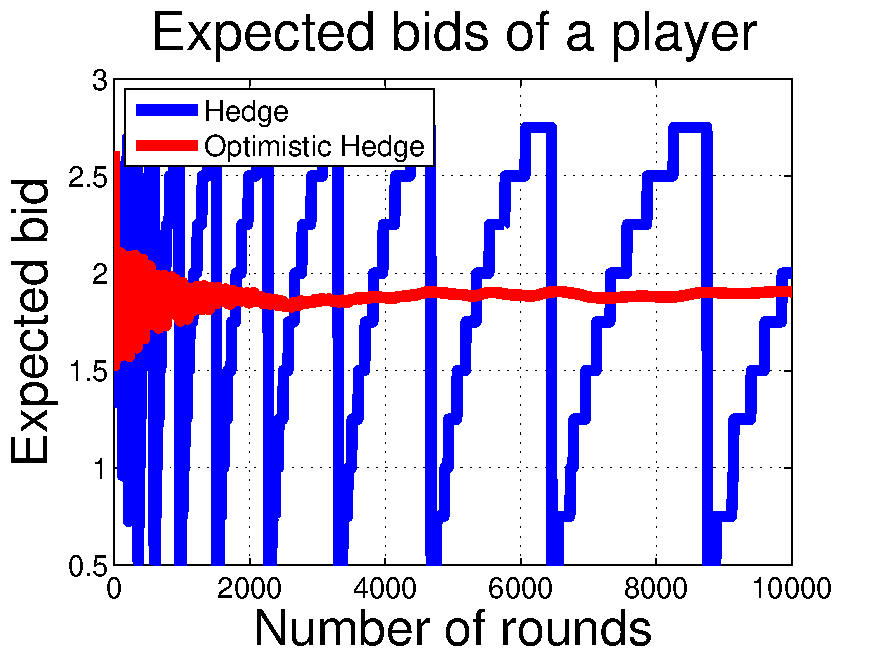
\includegraphics[width=0.4\textwidth,height=0.3\textwidth]{expected_bid.pdf}
		}
		\quad
		\subfigure{
			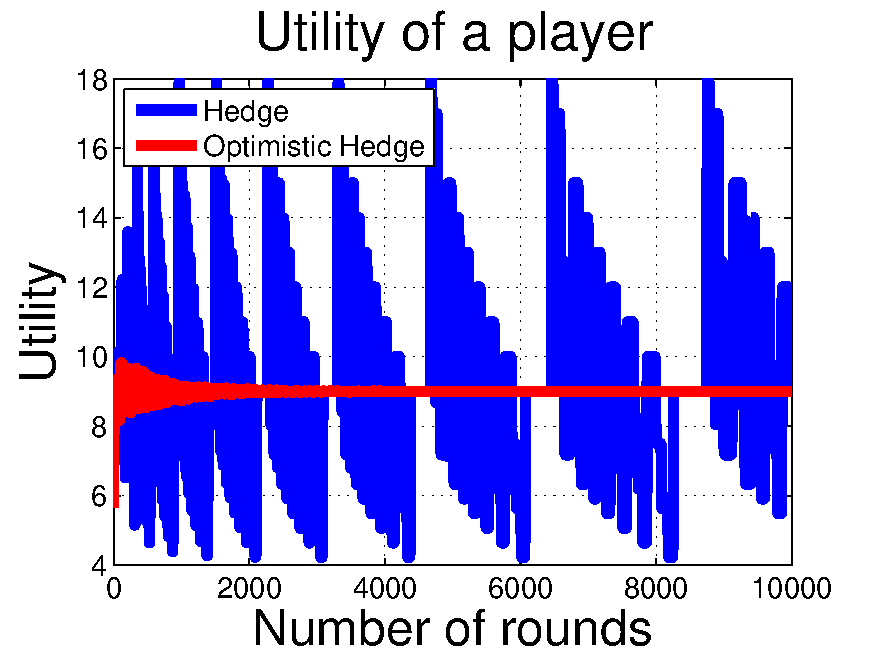
\includegraphics[width=0.4\textwidth,height=0.3\textwidth]{utilities.pdf}
		}
		\caption{Expected bid and per-iteration utility of a player on one of
			the four items over time, under Hedge (blue) and {Optimistic Hedge}
			(red) dynamics.}\label{fig:bids}
	\end{figure}
\end{frame}
\section{Discussion}
\subsection{Discussion}
\begin{frame}
	\frametitle{Discussion}
	\begin{itemize}
		\item Is \myprop~ necessary? (probably not)
		\item Is observing only the other's players moves instead of the expected utilities also enough to get faster rates?
		\item A precise quantification of the desired behaviour, which is necessary for stable trajectories, is of great interest.
	\end{itemize}
\end{frame}
% is RVU needed? probably not

\end{document}
